\documentclass{jarticle}

\usepackage{twocolumn}
%\usepackage[dvi ps]{graphicx}%%画像を読み込む
\usepackage[dvipdfmx]{graphicx}
\usepackage{subfigure}
\usepackage{amsmath}          %%genfrac http://www.biwako.shiga-u.ac.jp/sensei/kumazawa/tex/form006.html
\usepackage{ulem}             %%http://biwako.shiga-u.ac.jp/sensei/kumazawa/tex/ulem.html     uline,uuline,uwave,sout,xoutなど
\usepackage{multirow}
\usepackage{here}
%\usepackage{setspace}
\usepackage{chukan2018}       %%最後に読み込むこと!(最後に読み込まないと\textwidthなどの設定が反映されない)

\pagestyle{empty} %ページ番号を入れるときにはコメントアウトする

\begin{document}

\linesparpage{50}

\title{
カニ模倣型ロボットの開発に向けた細径空圧筋の改良
}
\etitle{
Improvement of Thin Pneumatic Muscles for Development of Crab-type Robot
}
\author{
研究者 濱口 紘生  指導教員  中西 大輔
}
\eauthor{
Keywords: McKibben Pneumatic Actuater, Exoskeleton, Biomimetic Robot
}

\maketitle

\thispagestyle{empty}  %1ページ目にページ番号を入れるときにはコメントアウトする

%%%%%%%%%%%%%%%%%%%%%%%%%%%%%%%%%%%%%%%%%%%%%%%%%%%%%%%%%%%%%%%%%%%%%%%%%%%%%%%
\section{緒言}

代表的な人工筋肉として,圧縮空気を印加することにより骨格筋のように収縮するMcKibben型人工筋肉(MPA)があげられる.
従来は直径が数十mm程度のものが多かったが,近年では数mm程度のMPAが注目を集めている\cite{wakimoto}.
その細さを活かして小さい筋肉,あるいは集積によって複雑な筋肉を表現可能なことから,筋骨格系ロボットに盛んに用いられている\cite{wakimoto}.
一方で,甲殻類のような外骨格を有する生物模倣ロボットでは,アクチュエータの配置が困難なことからワイヤ駆動や関節にサーボモータを配置したものが主流であった\cite{crabrobot1}.
細径MPAであれば骨格内部にアクチュエータを配置することが可能であり,実際の生物に近い構成でロボットを作成することが可能である.そこで本研究では外骨格生物のうち甲殻類の蟹をモデルに,
実際の蟹の筋肉と関節の構造を参考にして細径MPAを使用した蟹の歩脚ロボットの開発に取り組む.

%%%%%%%%%%%%%%%%%%%%%%%%%%%%%%%%%%%%%%%%%%%%%%%%%%%%%%%%%%%%%%%%%%%%%%%%%%%%%%%
\vspace*{-2mm}
\section{細径MPAを用いた羽状筋の再現}
\vspace*{-1mm}
\subsection{羽状筋について}
羽状筋とは,筋肉全体が斜めの角度で腱に付着する筋肉形状を指す.
この構造により,筋肉全体が羽のような配置を持ち,同じ断面積内に多くの筋繊維を収めることが可能となる.これにより,高い力を発生する特性を有する.
羽状筋は多くの生物に見られる筋配置の1つであり,人においては三角金がその代表例として挙げられる.
本研究で作製するカニ模倣型ロボットにおいても,外骨格内部に羽状筋に類似した筋構造を組み込む設計を行う.
%%%%%%%%%%%%%%%%%%%%%%%%%%%%%%%%%%%%%%%%%%%%%%%%%%%%%%%%%%%%%%%%%%%%%%%%%%%%%%%
\vspace*{-1mm}
\subsection{先行研究の課題と改良方法}

先行研究では図\ref{fig:OringMPA}上のように,MPAを構成するシリコンチューブとスリーブを端部で糸で縛り接着剤で固定する方式を採用していたが,
糸の締結に時間と練度を必要とすることや,度々空気漏れを生じるという難点があった.そこで本研究では端部部品を改良し,ゴムと端部を接着剤で,
スリーブと端部をOリングと接着剤でそれぞれ固定する方式へと変更した(図\ref{fig:OringMPA}下).これにより細径MPAに練度が不要となり,作成時間も大幅に短縮された.

続いて細径MPAの収縮性能向上に取り組んだ.
先行研究において開発された細径MPAにおいては,折癖の影響からスリーブが多少膨らんだ状態で作成されていたため,
圧力印加時の収縮量が減少してしまっていた.本研究ではメッシュの中に直径2mmの丸棒を差し込んで固定した状態でホットプレートで加熱することで熱可塑変化させた.
折癖をとるとともにスリーブの初期直径を2mmにまで小さくすることに成功し,収縮量を向上させることができた.

最後に,細径MPAを羽状配置するために端部の部品の構造を改良した.羽状筋は収縮した際に筋肉の角度が変化するが,先行研究では
根元の角度が固定されており,腱の引き込みの妨げになっていた.そこで本研究では図\ref{fig:MPAparts}の細径MPAの端部の部品を作成した.
図\ref{fig:MPAparts}の赤い斜線部の穴を回転の軸にして細径MPAの角度を自由に変化することができ,これにより細径MPA動作時に端部の部品に干渉しないことが確認できた.

%\begin{figure}[H]
%  \begin{minipage}[b]{0.47\columnwidth}
%    \centering
%    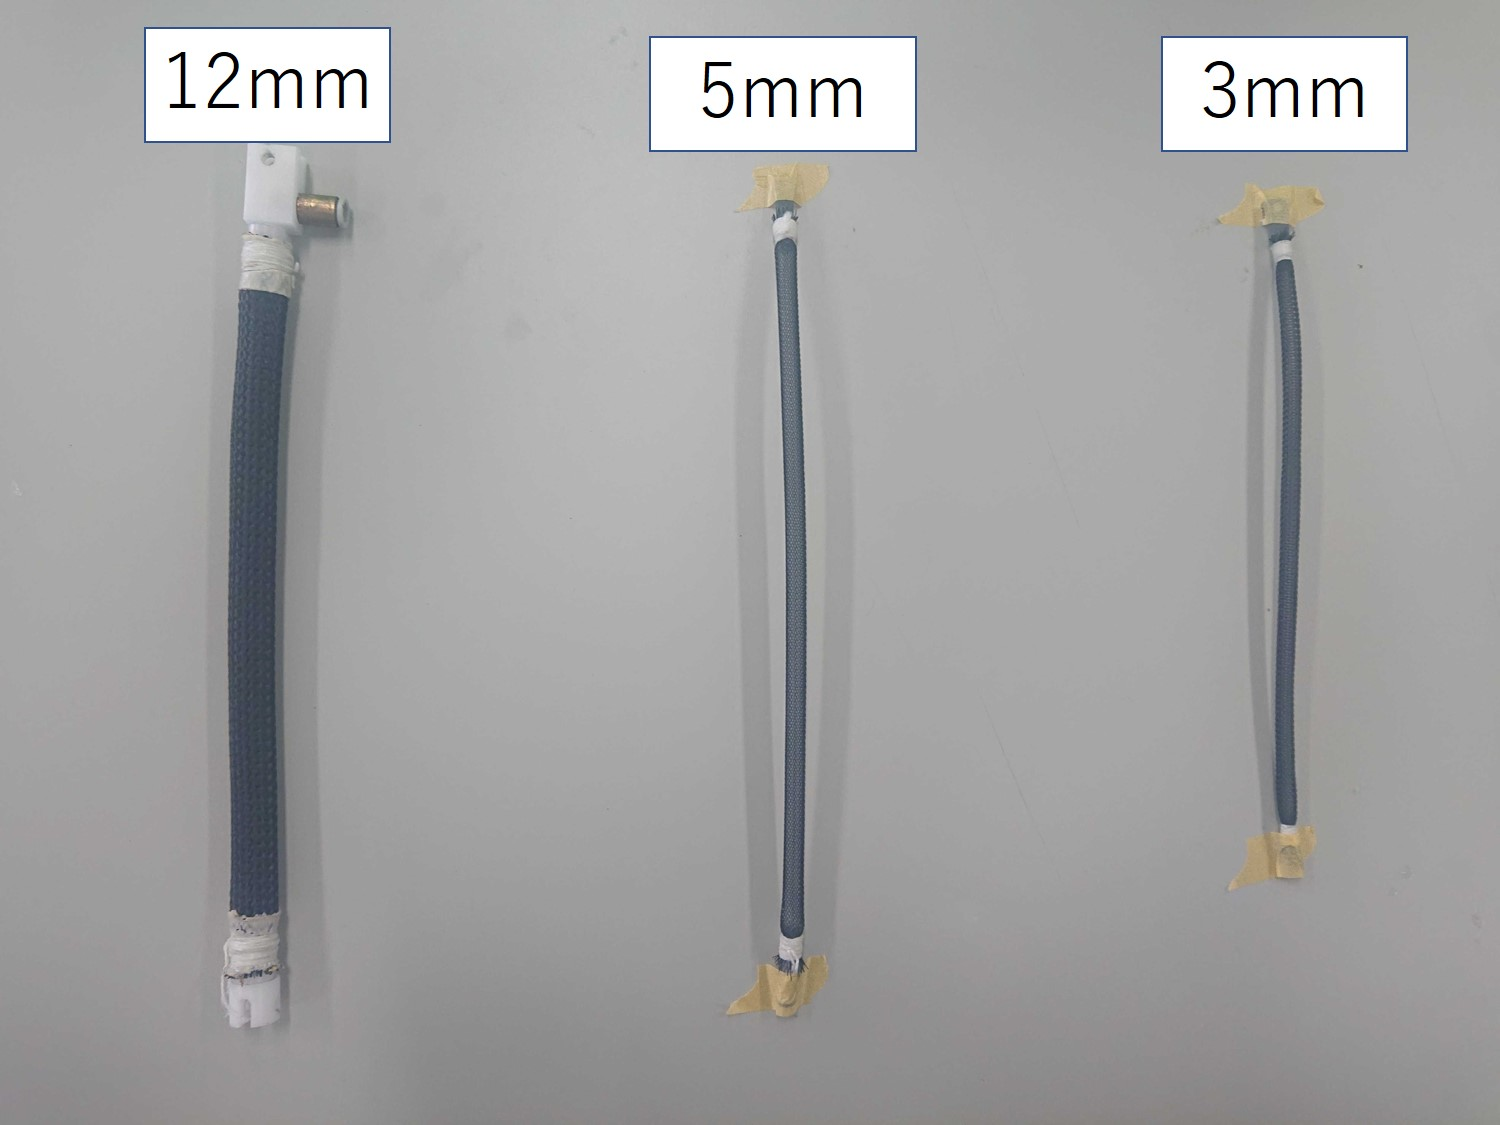
\includegraphics[scale=0.13]{image/mpa.JPG}
%    \vspace{-4mm}
%    \caption{MPAの外径}
%    \label{fig:MPA}
%  \end{minipage}
%  \hspace{0.04\columnwidth}
%  \begin{minipage}[b]{0.47\columnwidth}
%    \centering
%    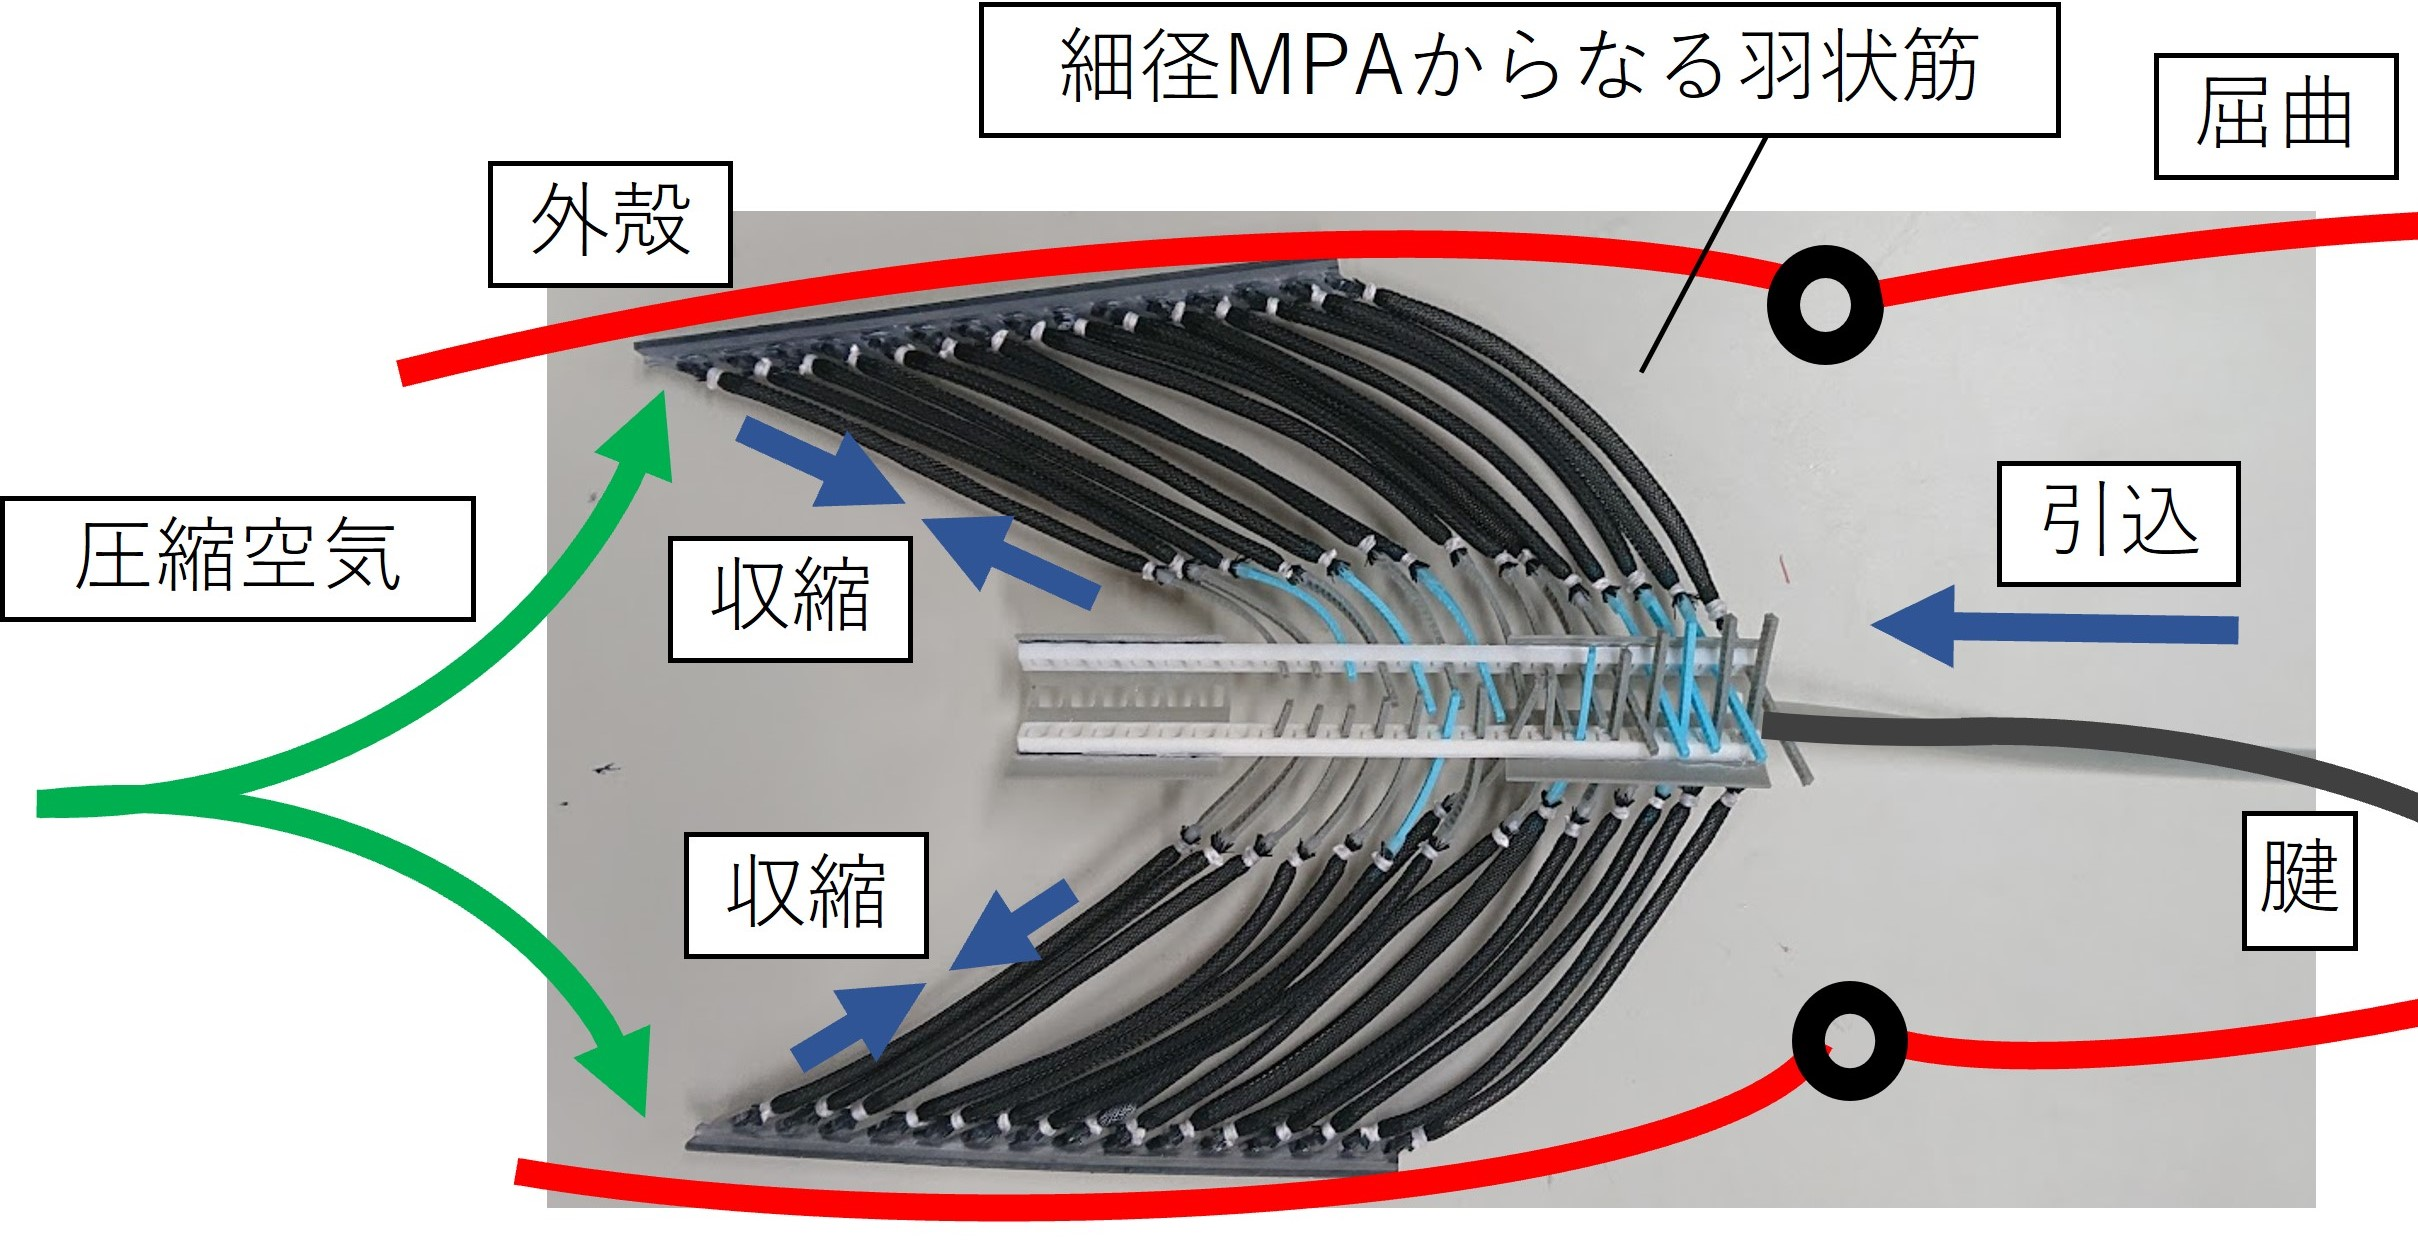
\includegraphics[scale=0.19]{image/mosiki.JPG}
%    \vspace{-6mm}
%    \caption{蟹模倣ロボット\cite{crabrobot2}}
%    \label{fig:crabrobot}
%  \end{minipage}
%\end{figure}
%\vspace*{-5mm}
\begin{figure}[t]
  \begin{minipage}[b]{0.47\columnwidth}
    \centering
    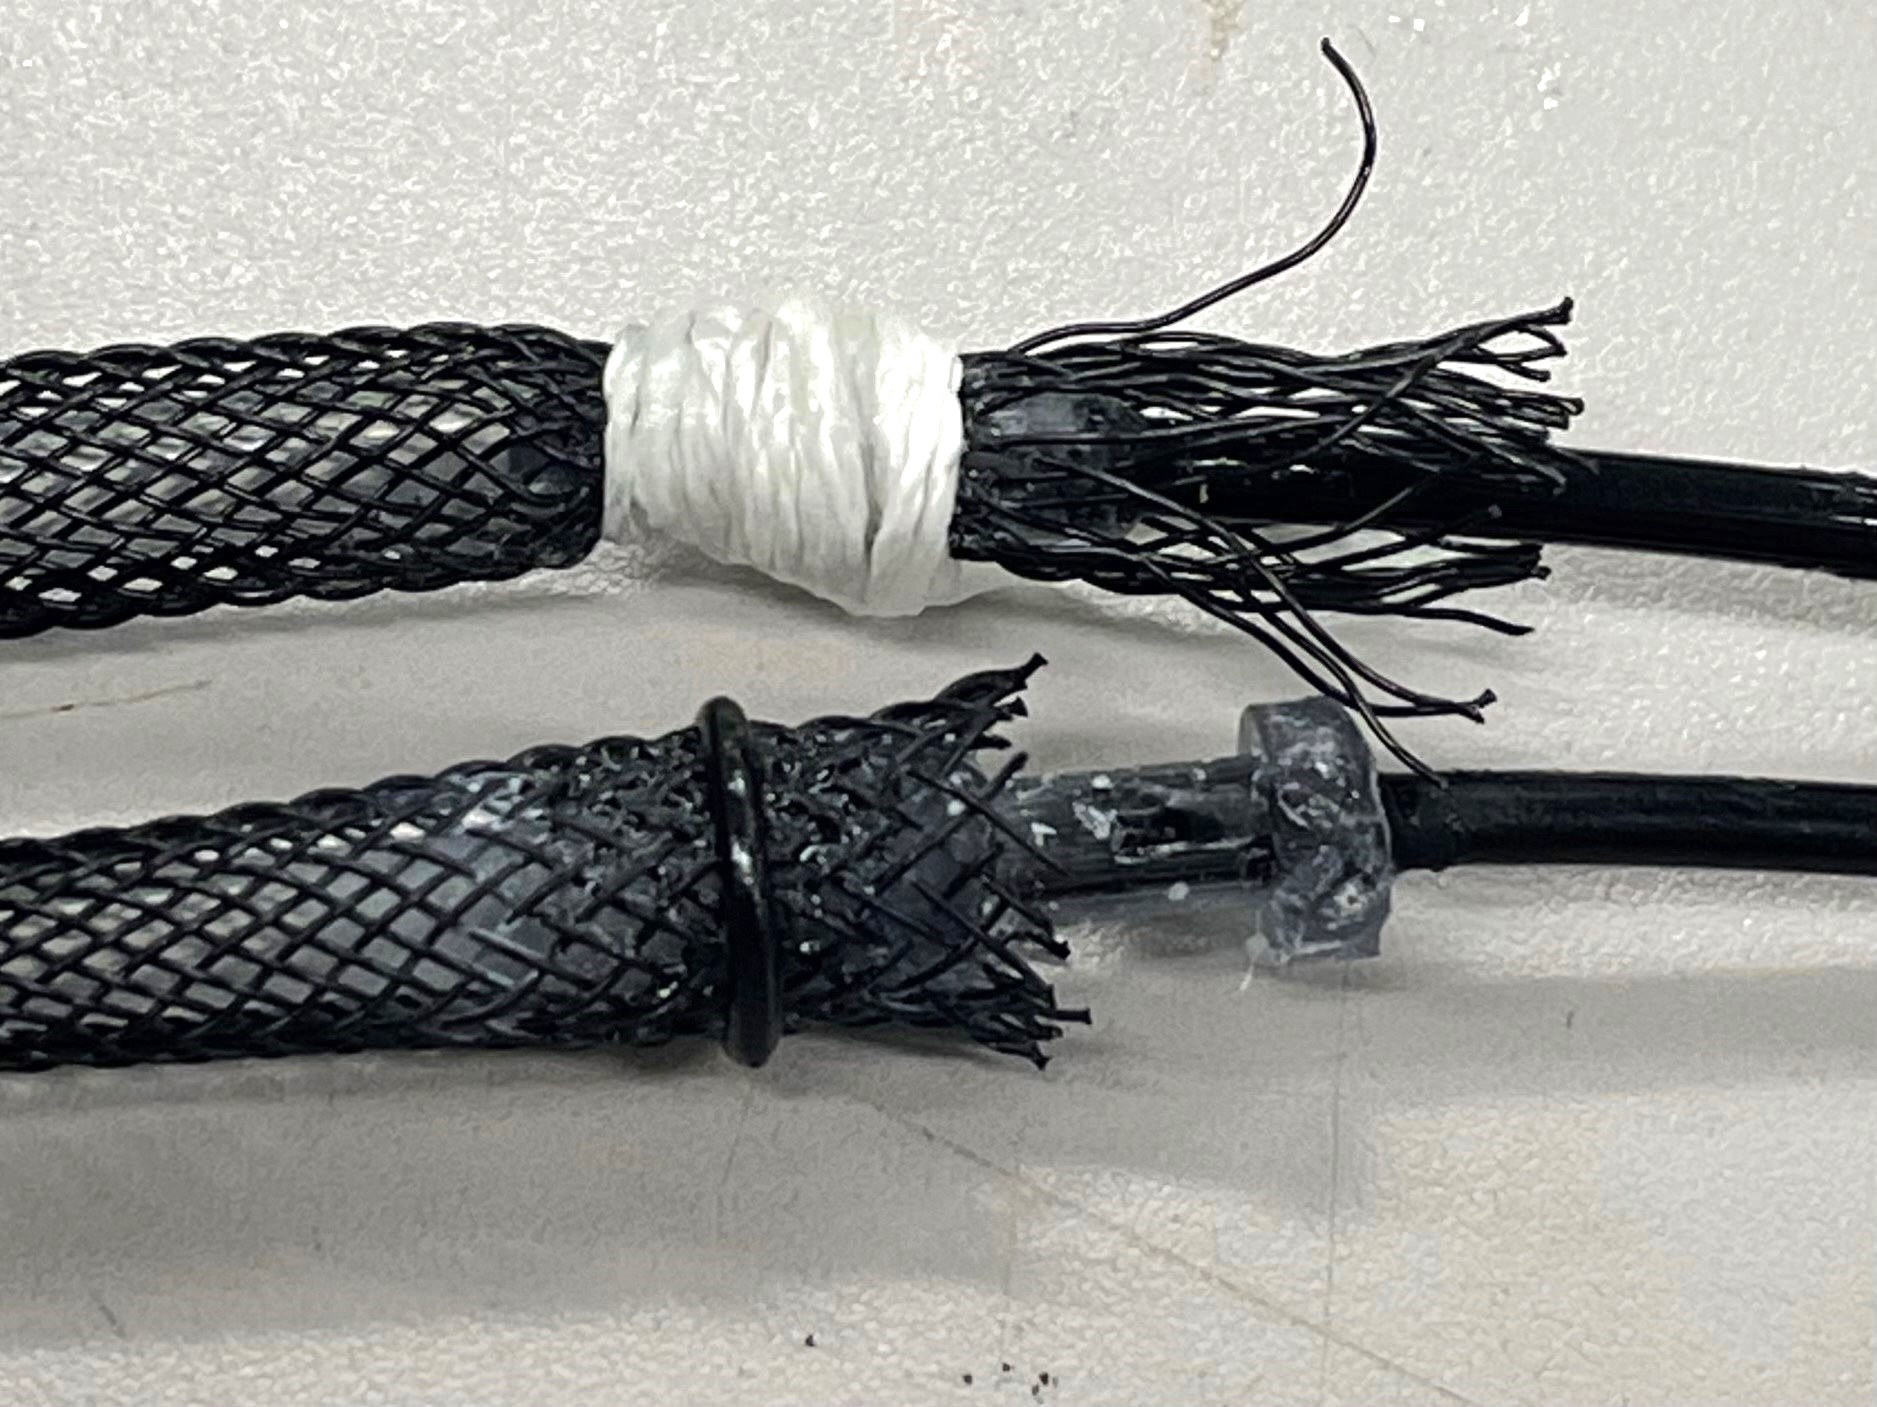
\includegraphics[scale=0.05]{image/mpa_oring_1.jpg}
    \vspace{-2mm}
    \caption{細径MPA締結方法}
    \label{fig:OringMPA}
  \end{minipage}
  \hspace{0.04\columnwidth}
  \begin{minipage}[b]{0.47\columnwidth}
    \centering
    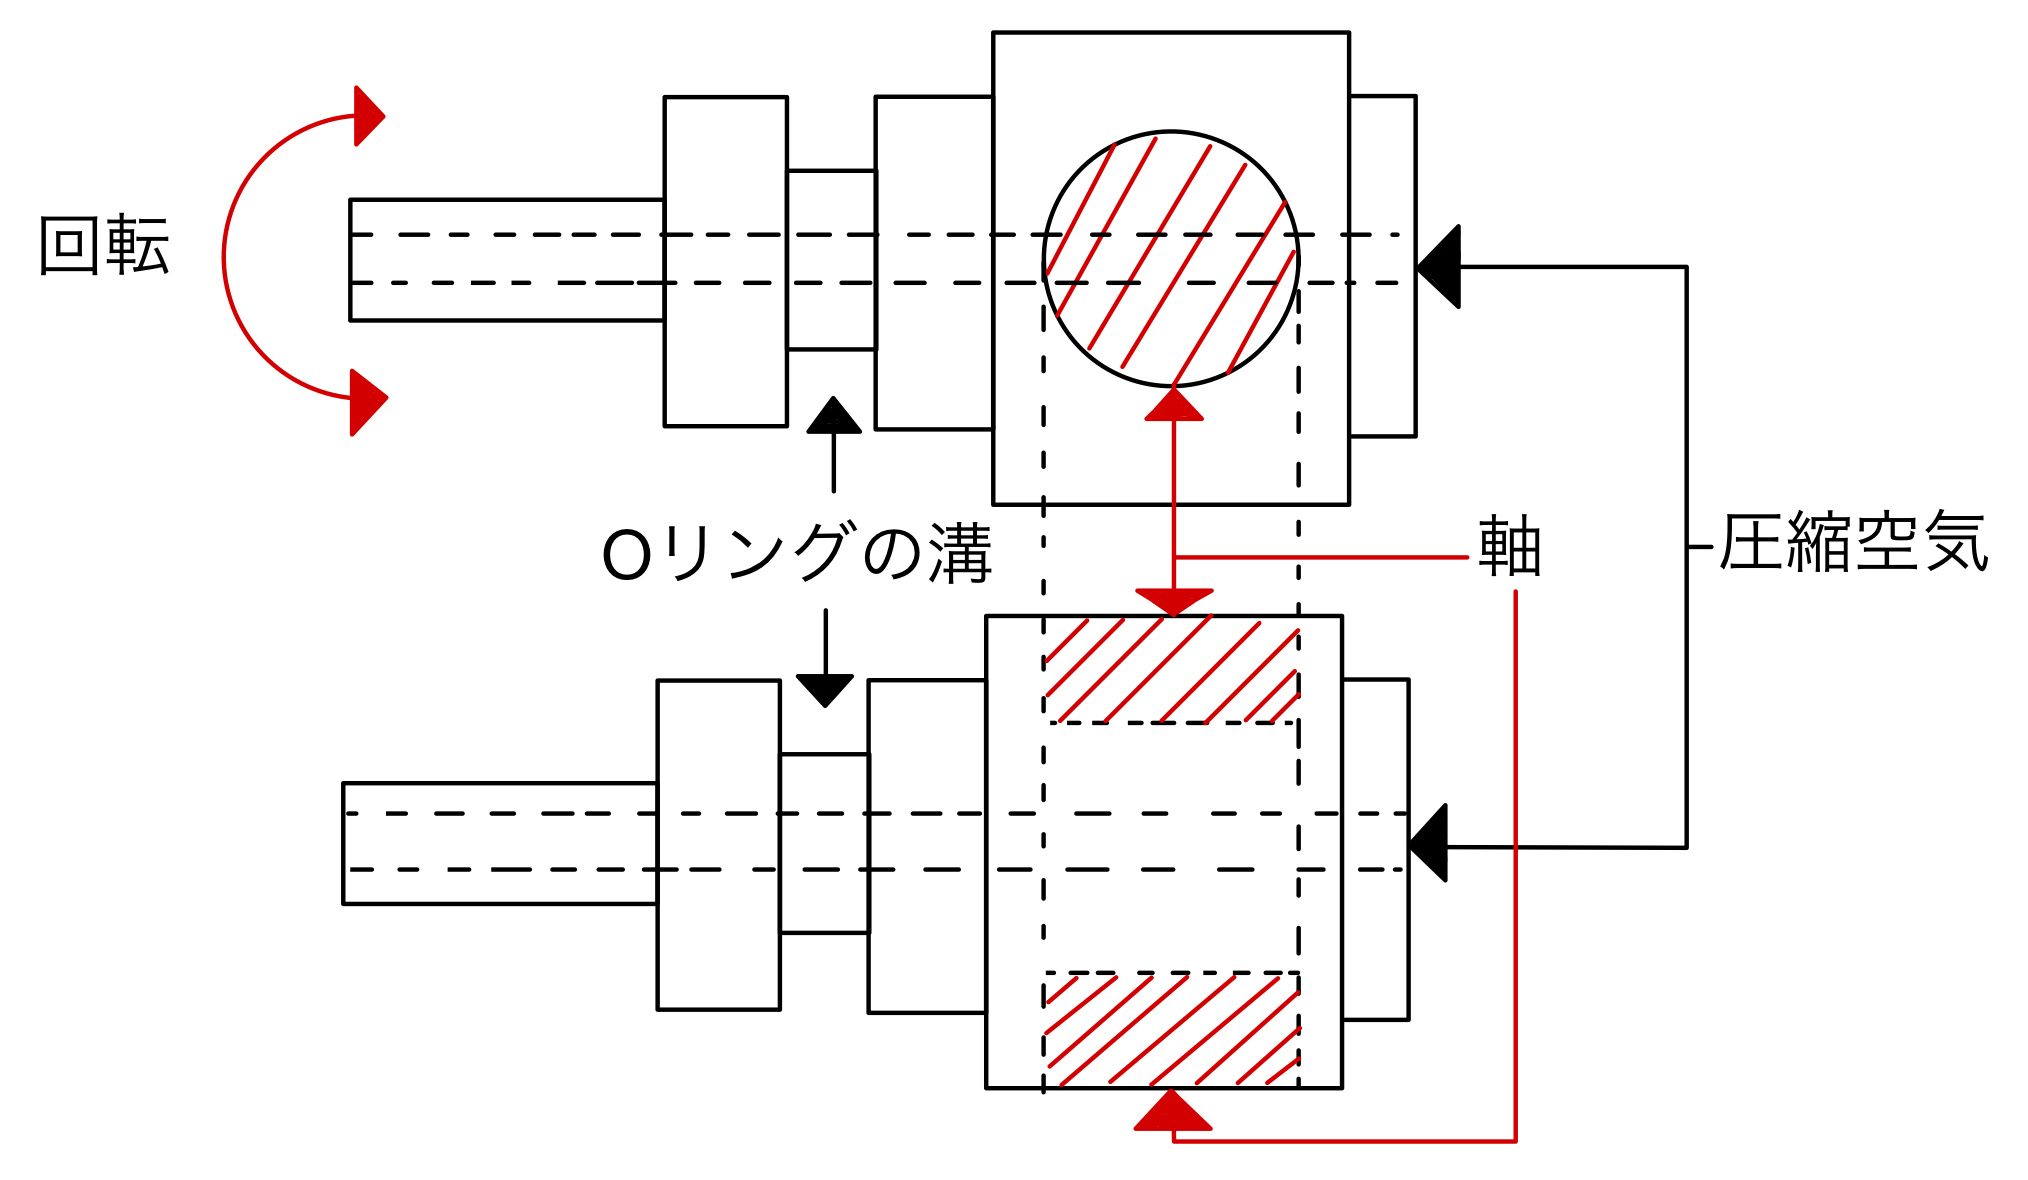
\includegraphics[scale=0.047]{image/MPA_irast.jpg}
    \vspace{-2mm}
    \caption{細径MPA端部部品}
    \label{fig:MPAparts}
  \end{minipage}
\end{figure}
%%%%%%%%%%%%%%%%%%%%%%%%%%%%%%%%%%%%%%%%%%%%%%%%%%%%%%%%%%%%%%%%%%%%%%%%%%%%%%%
\vspace*{-2mm}
\section{実機の設計・作成方法}
\vspace*{-1mm}
\subsection{外骨格の設計について}

作成した実機を図\ref{fig:jikki}に示す.
今回の研究では甲殻類のうち蟹のズワイガニの歩脚モデルに機体を作成した.
機体作成時には先行研究\cite{crabrobot2}のズワイガニの歩脚の各部寸法と,本研究で新たに解剖した際に得られた可動域をもとにしてモデリングした.
ただし機体内部に細径MPAや腱部品などを配置する必要があるため,実測値に対して直径方向には7倍,長手方向には3.5倍のサイズとした.
可動域を実際の蟹に近づけるために腕節部だけ長手方向に6.3倍した.
作成にはMPA方式の3Dプリンタを使用し,関節部にはベアリングを入れている.
長手方向の具体的な寸法としては,長節が350 mm,腕節が256 mm,前節が245 mm,指節が100 mmである.
%%%%%%%%%%%%%%%%%%%%%%%%%%%%%%%%%%%%%%%%%%%%%%%%%%%%%%%%%%%%%%%%%%%%%%%%%%%%%%%
\vspace{-1mm}
\subsection{細径MPAを用いた羽状筋の再現について}

本研究では,羽状筋のような蟹の駆動機構を再現するため細径MPAを用いた羽状筋の開発を行った.開発した羽状筋を図\ref{fig:muscle}に示す.
上記で説明した羽状筋の筋繊維は1本ずつ長さが異なっているが,作成方法と関節の可動域の幾何学的計算を簡易化するため図\ref{fig:muscle}のように細径MPAの長さがすべて等しくなるように設計した.
図\ref{fig:muscle}の細径MPAの端部にある黒い部品は3章で紹介した細径MPAの収縮に合わせて角度が自由に変化でき,圧縮空気を各細径MPAへ一度に供給することができる部品である.この部品は光造形方式の3Dプリンターで作製した.
また図\ref{fig:muscle}にある灰色の部品は蟹の腱を模したもので,TPU素材を使用してFDM方式の3Dプリンターで作製したので柔軟性が高くねじれに対応可能である.
腱と外骨格は全てねじで固定しており,腱の張り具合は可能な仕組みになっている.

実際の蟹の可動域を再現するために必要な腱のストローク,細径MPAの配置が理由で可動域を再現不可能な関節の可動域を幾何学的計算から求めた(表\ref{tab:kadouiki}).
%%%%%%%%%%%%%%%%%%%%%%%%%%%%%%%%%%%%%%%%%%%%%%%%%%%%%%%%%%%%%%%%%%%%%%%%%%%%%%%
\vspace*{-4mm}
\begin{figure*}[t]
  \centering
  \subfigure[長節-腕節間の動作実験]{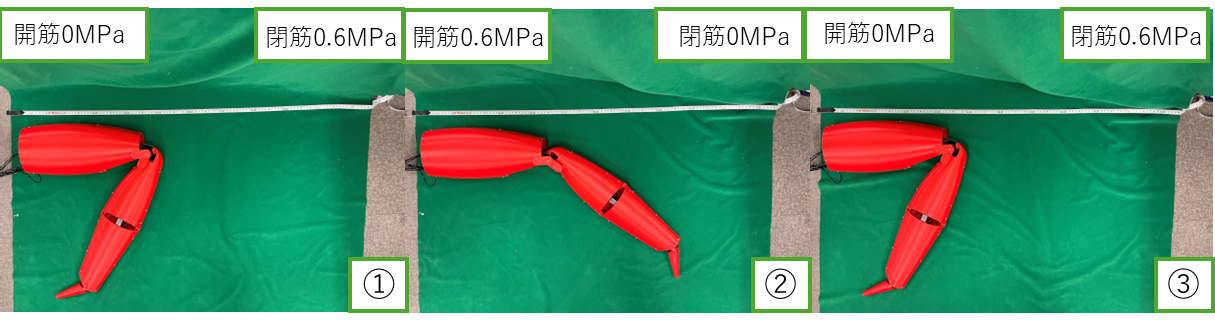
\includegraphics[scale=0.24]{image/chousetu-wansetu_edited.png}}\\
  \label{fig:move1}
  \vspace{-2mm}
  \subfigure[腕節‐前節間の動作実験]{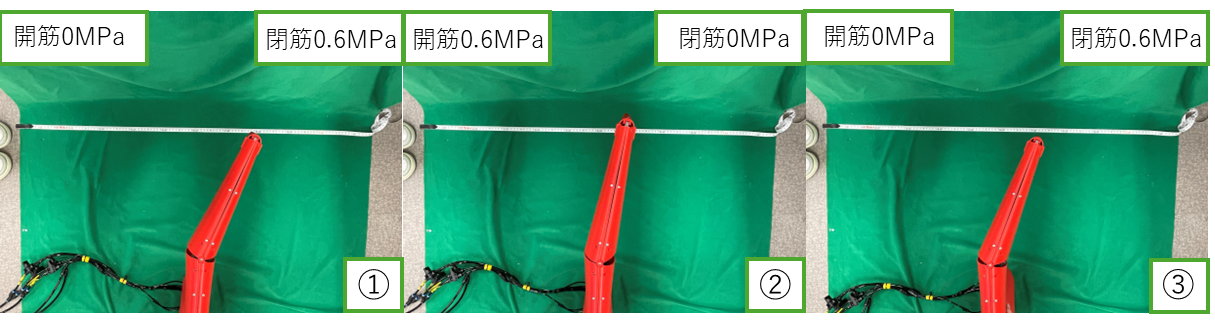
\includegraphics[scale=0.24]{image/wansetu-zensetu_edited.png}}\\
  \label{fig:move2} 
  \vspace{-2mm}
  \subfigure[前節‐指節間の動作実験]{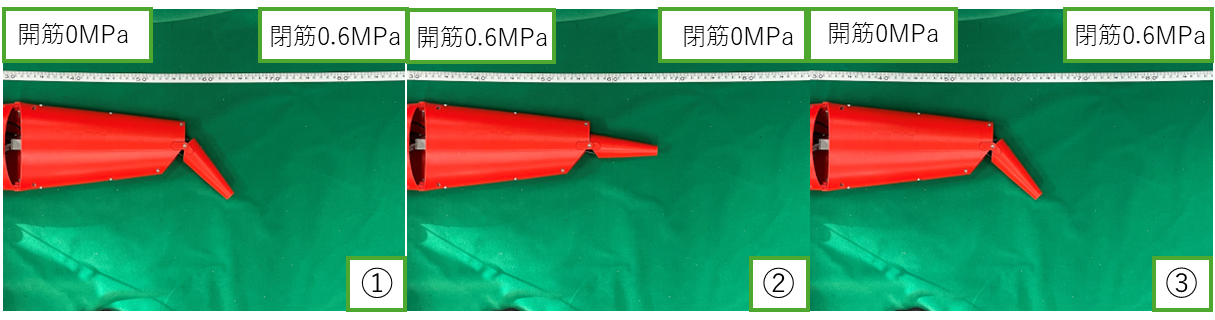
\includegraphics[scale=0.24]{image/zensetu-sisetu_edited.png}}\\
  \label{fig:move3} 
  \vspace{-2mm}
  \caption{動作実験の様子.ここで開筋は関節を開く方向に,閉筋は閉じる方向に作用する羽状筋を指す.}
  \label{fig:jikken}
  \vspace{-2mm}
\end{figure*}
%%%%%%%%%%%%%%%%%%%%%%%%%%%%%%%%%%%%%%%%%%%%%%%%%%%%%%%%%%%%%%%%%%%%%%%%%%%%%%%
%\begin{eqnarray}
%	\label{theta2} \theta_2 &=& \sin^{-1}\left(\frac{d}{0.8 \ell_1}\right)\\
%  \label{Se} S_e &=& \ell_1 \cos\theta_1 - \ell_2 \cos\theta_2
%\end{eqnarray}
%%%%%%%%%%%%%%%%%%%%%%%%%%%%%%%%%%%%%%%%%%%%%%%%%%%%%%%%%%%%%%%%%%%%%%%%%%%%%%%
\vspace*{-2mm}
\section{動作実験}

長節から指節にかけてMPAを配置し動作実験を行った.関節の動きを確認しやすくするために長節-腕節間と前節-指節間は機体を寝かせた状態,腕節-前節間は機体を立てた状態で動作実験を行った.
また,初期位置は開筋か閉筋のどちらか一方が張った状態の位置にし,圧縮空気の印加は手動で行い印加圧力は0.6MPa,開筋と閉筋の手動弁を交互に開閉することで動作させた.

長節-腕節間の動作結果を図\ref{fig:move1},腕節-前節の動作実験を図\ref{fig:move2},前節-指節の動作実験を図\ref{fig:move3}に示す.
結果より,長節-腕節間では初期状態(図\ref{fig:move1}左)と最終状態(図\ref{fig:move1}右)では歩脚の角度が近い状態になった.
腕節-前節間,前節-指節間では長節-腕節間と同じような動きがみられたが,可動域が少し狭く感じた.

また,動作分析ソフトウェアのKinoviaと数値解析が可能なMATLABを用いて実機の可動域を計測した(表\ref{tab:kadouiki}).
その結果,長節-腕節間では実際の可動域の再現することができた.
腕節-前節間は実際の蟹の可動域は再現できていなかったが,今回設計した実機で出力可能な可動域を再現できていた.
前節-指節間は今回の設計では実際の蟹の可動域が再現可能にもかかわらず,実際の蟹の半分の可動域しか再現できていなかった.
%%%%%%%%%%%%%%%%%%%%%%%%%%%%%%%%%%%%%%%%%%%%%%%%%%%%%%%%%%%%%%%%%%%%%%%%%%%%%%%
\vspace*{-2mm}
\section{考察}

前節-指節間の関節の動きが小さい原因について考察する.
考察は細径MPAが全て同じ長さで作成することができなかったことと,前節-指節間では閉筋に圧縮空気を印加した際に,腱付着点から節の中心に向かって伸びている腱の長さが他の関節に比べて長かった.
それにより本来のストロークを出し切れていなかった.などについて考察していきたいと考えています.

%\begin{figure}[t]
%    \centering
%   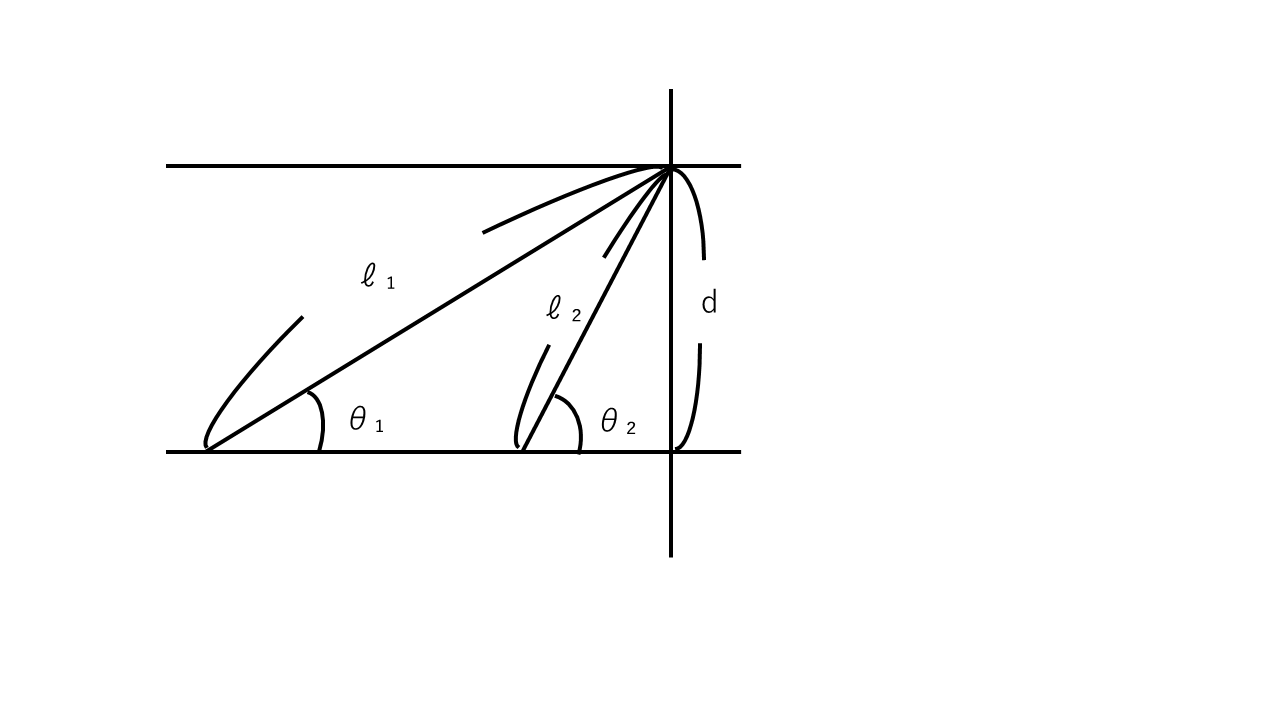
\includegraphics[scale=0.18]{image/keisan_1.png}
%    \vspace{-4.5mm}
%    \caption{実機の簡易モデル}
%    \label{fig:keisan_1}
  %\end{minipage}
%\end{figure}
%%%%%%%%%%%%%%%%%%%%%%%%%%%%%%%%%%%%%%%%%%%%%%%%%%%%%%%%%%%%%%%%%%%%%%%%%%%%%%%
\begin{figure}[!t]
  \begin{minipage}[b]{0.47\columnwidth}
    \centering
    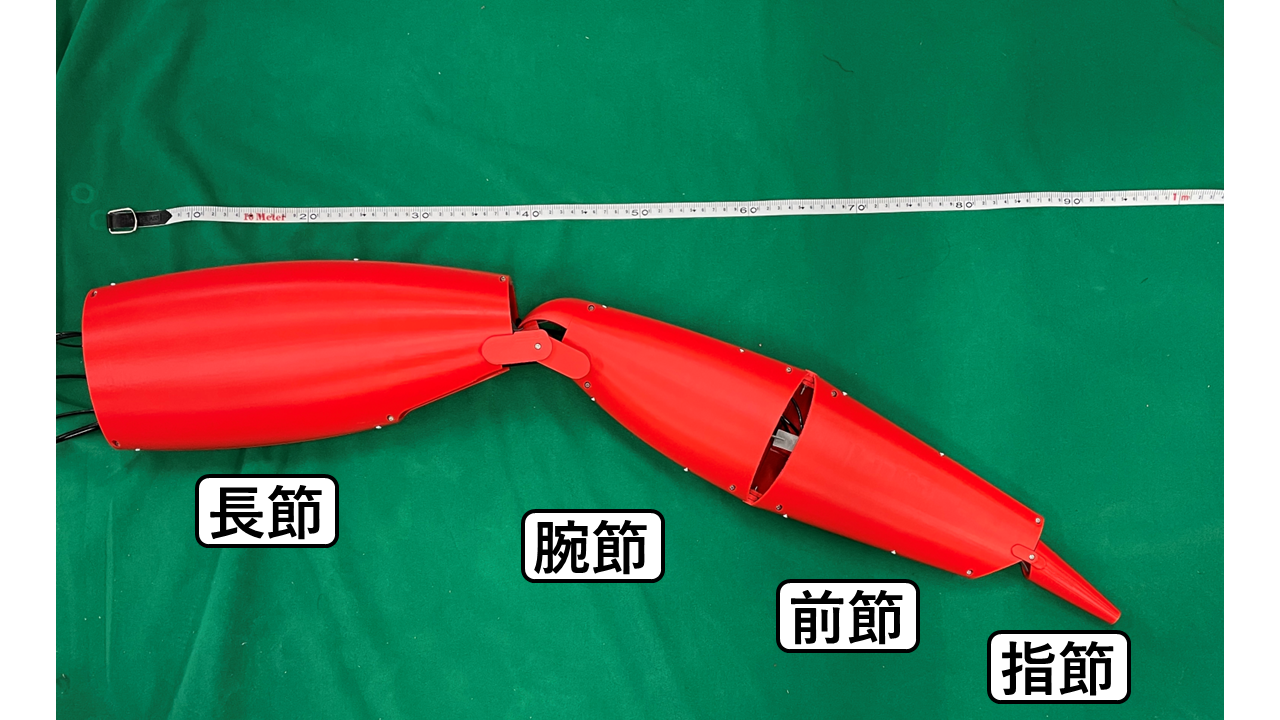
\includegraphics[scale=0.1]{image/jikki.png}
    \vspace{-2mm}
    \caption{実機の外観}
    \label{fig:jikki}
  \end{minipage}
  \hspace{0.04\columnwidth}
  \begin{minipage}[b]{0.47\columnwidth}
    \centering
    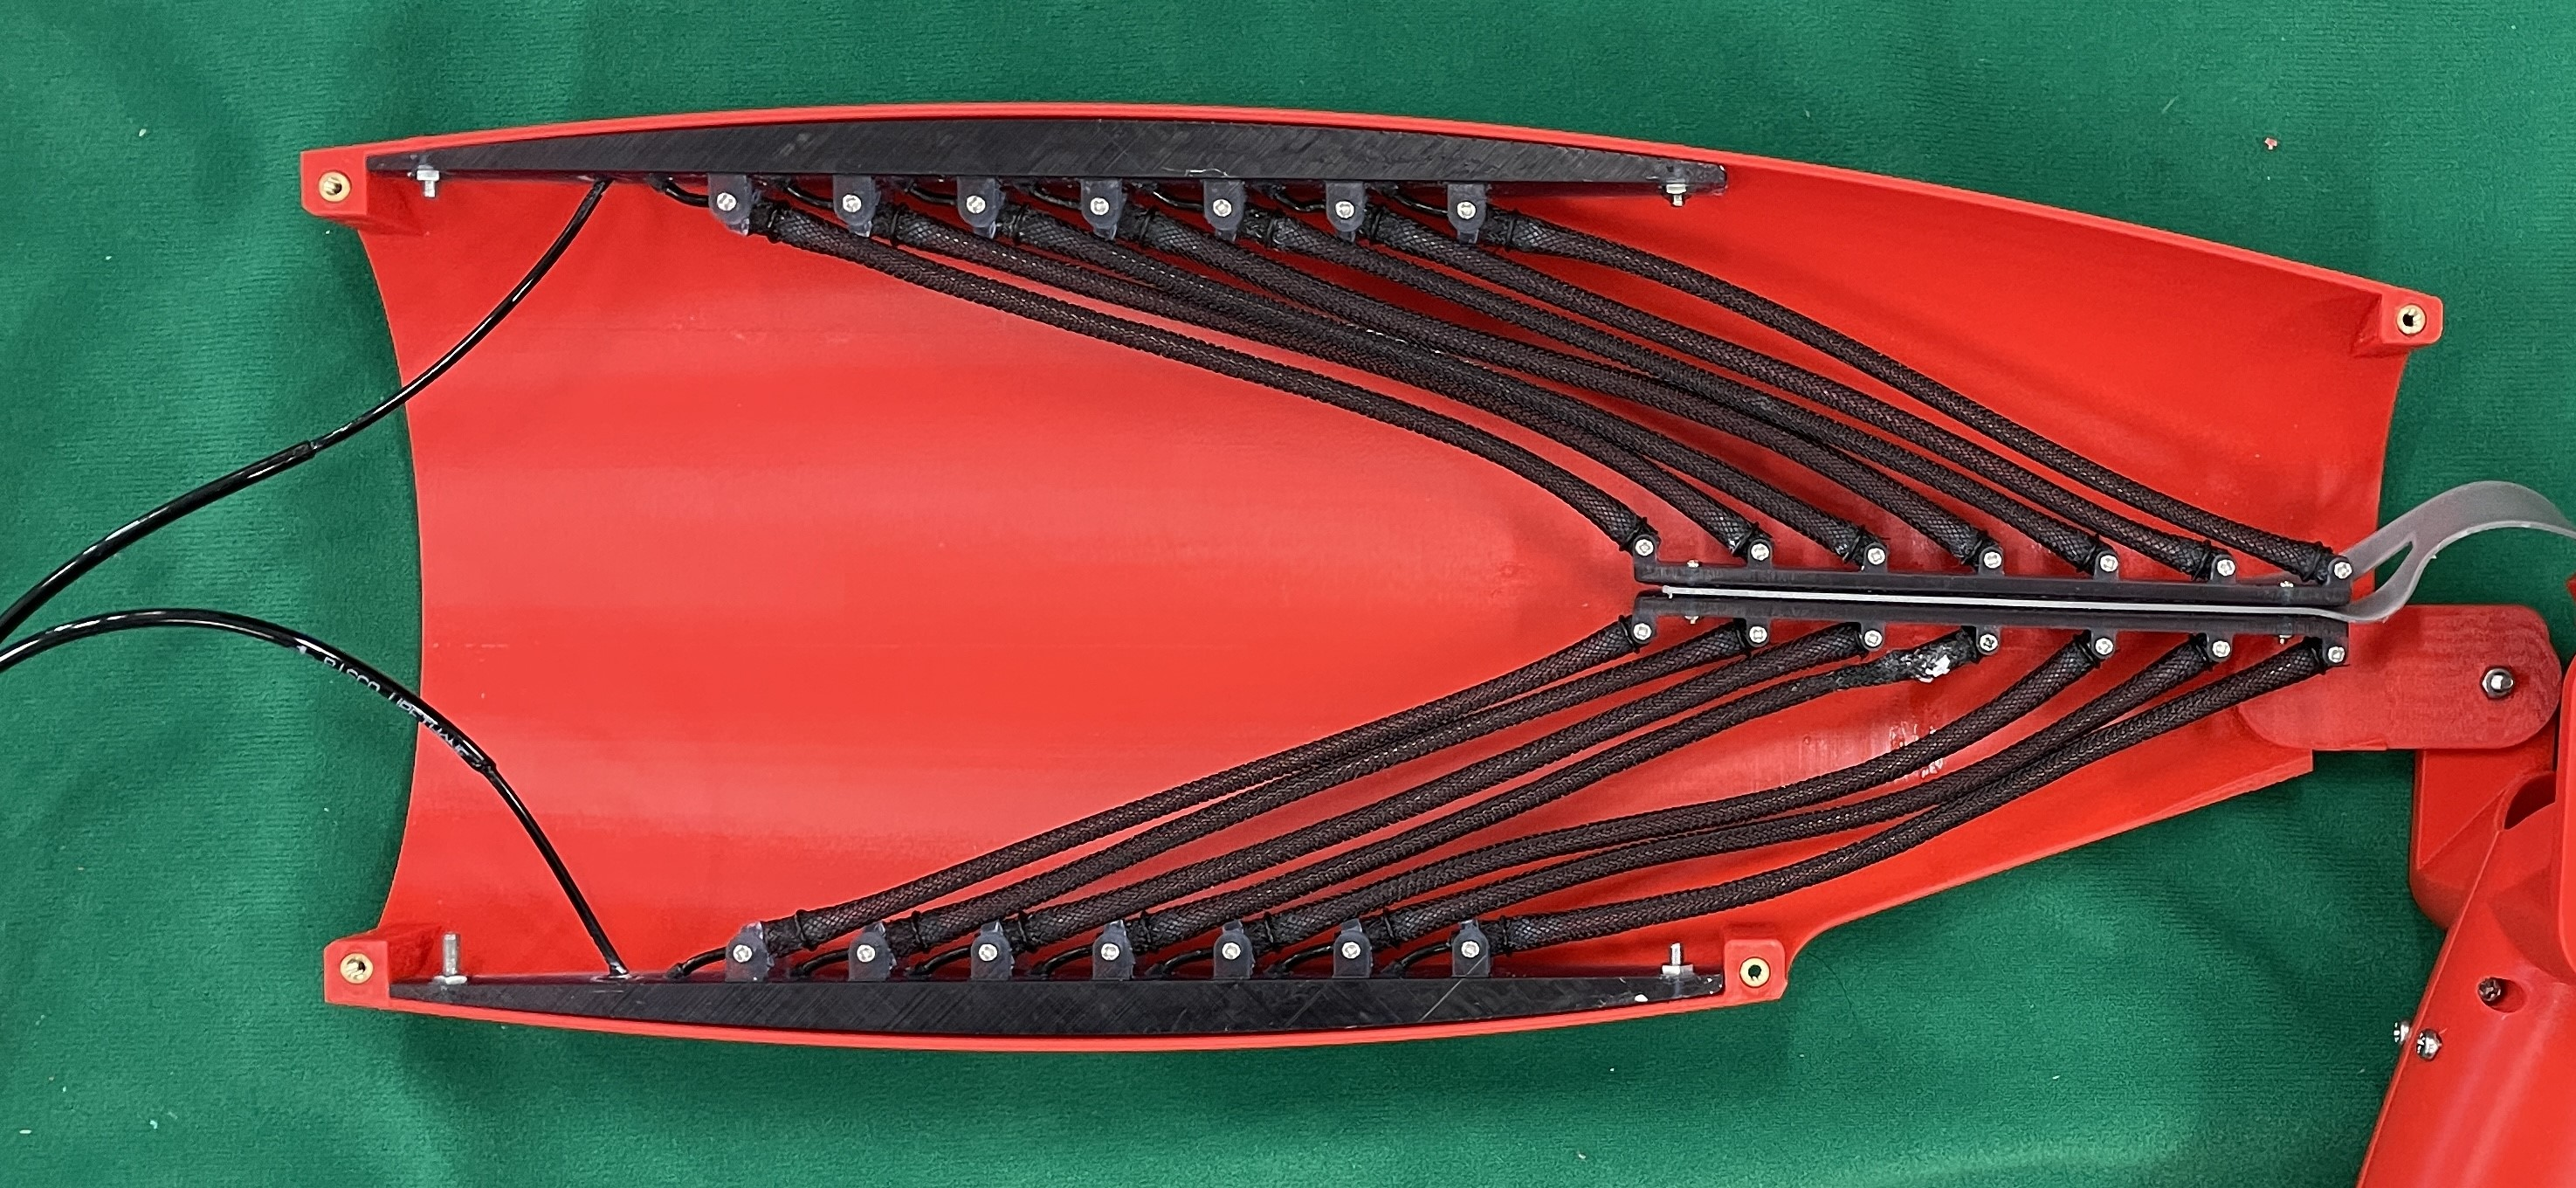
\includegraphics[scale=0.03]{image/crabmuscle.jpg}
    \vspace{1mm}
    \caption{実機内部の筋配置}
    \label{fig:muscle}
  \end{minipage}
\end{figure}
%%%%%%%%%%%%%%%%%%%%%%%%%%%%%%%%%%%%%%%%%%%%%%%%%%%%%%%%%%%%%%%%%%%%%%%%%%%%%%%
\begin{table}[!t]
  \centering
  \vspace{-2mm}
  \caption{実際の蟹と実機の可動域比較}
  \vspace{1mm}
  \scalebox{0.68}{ 
      \begin{tabular}{|c|c|c|c|}
          \hline
          項目/部位 & 長節-腕節間 & 腕節-前節間 & 前節-指節間 \\ \hline
          実際の蟹の可動域 & 52$\sim$130 & 0$\sim$45 & 0$\sim$89 \\ \hline
          計算上のロボットの可動域 & 45.3$\sim$133.1 & 3.25$\sim$36.0 & 9.82$\sim$39.8 \\ \hline
          実際のロボットの動域 & 45.3$\sim$133.1 & 3.25$\sim$36.0 & 9.82$\sim$39.8 \\ \hline
      \end{tabular}
  }
  \label{tab:kadouiki}
\end{table}

%%%%%%%%%%%%%%%%%%%%%%%%%%%%%%%%%%%%%%%%%%%%%%%%%%%%%%%%%%%%%%%%%%%%%%%%%%%%%%%
\vspace*{-2mm}
\section{結言}
本稿では,外骨格生物模倣ロボットの開発をするにあたって課題となる細径MPA の作成方法と固定方法について改良を行った.
さらにそれらを用いてカニ模倣型ロボットの開発に成功し,長節から指節までの動作実験を行った.
節の開閉動作を確認することができたが実際の蟹の可動域を完全に再現することはできなかった.
今後は細径MPAを同じ長さに配置する方法,動作時に腱が関節から離れない設計を考えることにより実際の蟹の動きに近づけるような歩脚ロボットの完成を予定している.

%%%%%%%%%%%%%%%%%%%%%%%%%%%%%%%%%%%%%%%%%%%%%%%%%%%%%%%%%%%%%%%%%%%%%%%%%%%%%%%
\begin{thebibliography}{99}
  \bibitem{wakimoto}
  脇本修一,
  細径McKibben型人工筋の開発と用途開拓,
  計測と制御,57巻,11号,pp.812-815,2018
  
  \bibitem{crabrobot1}
  CHEN, Xi, et al. Study on the Design and Experimental Research on a Bionic Crab Robot with Amphibious Multi-Modal Movement, Journal of Marine Science and Engineering,10,12,p.1804,2022
  
  \bibitem{crabrobot2}
  中西大輔,長谷川侑大,浪花啓右,杉本靖博,
  細径空圧筋を用いた羽状筋および外骨格生物模倣ロボットの開発,ロボティクス・メカトロニクス講演会2024,2A1-L08,2024.

  \bibitem{crab}
  D.Hazerli and S.Richter,
  Why“swimming crabs”are able to swim-The importance of the axial skeleton:A comparison between the“swimming crab”Liocarcinus depurator and two other brachyuran crabs (Cancer pagurus, Carcinus maenas) using μCT and 3D-reconstruction,
  Arthropod Structure&Development,
  59,p.100972,2022

 \end{thebibliography}
 %%%%%%%%%%%%%%%%%%%%%%%%%%%%%%%%%%%%%%%%%%%%%%%%%%%%%%%%%%%%%%%%%%%%%%%%%%%%%%%
\end{document}